% IEEE Paper Template for US-LETTER Page Size (V1)
% Sample Conference Paper using IEEE LaTeX style file for US-LETTER pagesize.
% Copyright (C) 2006 Causal Productions Pty Ltd.
% Permission is granted to distribute and revise this file provided that
% this header remains intact.
%
\documentclass[10pt,conference,letterpaper]{IEEEtran}
%\documentclass{IEEEtran}
\usepackage{url}
\usepackage{graphicx}
\usepackage{capt-of}
\usepackage{color}
\usepackage{lscape, subfigure, latexsym, amssymb, amsmath, algorithm, algorithmic}
\usepackage{eucal}
\usepackage{eufrak}
\newtheorem{defn}{Definition}
\usepackage{multirow}
\usepackage{tabularx}
\usepackage{epsf}
\usepackage{balance}
\usepackage{stmaryrd}
%\usepackage{appendix}
%\usepackage{pxfonts}
% names of approaches
% ----------------------------------------------------------------
%changes to the algorithm format
%\newcommand{\algorithmicreturn}{\textbf{return}}
%\newcommand{\algorithmiccomment}[1]{// #1}
\newcommand{\DoubleSpace}{\edef\baselinestretch{1.45}\Huge}
% \newcommand{\DoubleSpace}{\edef\baselinestretch{1.0}\Huge\normalsize}
\newcommand{\SingleSpace}{\edef\baselinestretch{1.0}\Huge\normalsize}
\newcommand{\eat}[1] {}
\newcommand{\reminder}[1]{\textcolor{red}{\em $\rightarrow$ (#1)$\leftarrow$}}
\newcommand{\remove}[1]{\textcolor{blue}{\em $\rightarrow$ [{\bf REM-START} (#1) {\bf REM-END}] $\leftarrow$}}

% \newcommand{\reminder}[1]{ [[[ \marginpar{\mbox{$<==$}} #1 ]]] }
% \newcommand{\reminder}[1]{ [[[{\underline{ \sl $\longrightarrow$ #1 $\longleftarrow$}}]]]}
%\newcommand{\BigCrunch}{}
%\newcommand{\Crunch}{}
%\newcommand{\SmallCrunch}{}
%\newcommand{\Skip}{}

\newcommand{\BigCrunch}{\vspace*{-1.5em}}
\newcommand{\Crunch}{\vspace*{-1em}}
\newcommand{\SmallCrunch}{\vspace*{-1ex}}
\newcommand{\Skip}{\vspace*{1ex}}


\newcommand{\myDefnBegin}[1]{
\SmallCrunch
\begin{defn} \label{#1}
}

\newcommand{\myDefnEnd}{
\end{defn}
\SmallCrunch
}

\newcommand{\myThmBegin}[1]{
%\Crunch
\begin{thm} \label{#1}
}

\newcommand{\myThmEnd}{
\end{thm}
%\BigCrunch
}

\newcommand{\customizedfig}[4]{
\begin{figure}[t]
\begin{center}
  \includegraphics[width=#4]{#1}\\
%  \vspace*{-1em}
  \caption{#2}\label{#3}
%  \vspace*{1em}
\end{center}
\BigCrunch
\end{figure}
}

\newcommand{\customizedfigInCol}[4]{
\begin{figure*}[t]
\begin{center}
  \includegraphics[width=#4]{#1}\\
%  \vspace*{-1em}
  \caption{#2}\label{#3}
%  \vspace*{1em}
\end{center}
\BigCrunch
\end{figure*}
}

\newcommand{\onesmallfigure}[3]{
%\Crunch
\begin{figure}[tb]
\begin{center}
\centerline{\epsfxsize=1.2in \epsffile{#1}}
% \DoubleSpace
%\SmallCrunch
\centerline{\parbox{7in}{\caption{#2} \label{#3}}}
%\BigCrunch
\end{center}
\BigCrunch
\end{figure}
}

\newcommand{\onemediumfigure}[3]{
%\Crunch
\begin{figure}[tb]
\begin{center}
\centerline{\epsfxsize=2.0in \epsffile{#1}}
% \DoubleSpace
%\Crunch
\centerline{\parbox{3in}{\caption{#2} \label{#3}}}
% \SingleSpace
\end{center}
\BigCrunch
\end{figure}
}


\newcommand{\onefigure}[3]{
\begin{figure}[t]
\begin{center}
\centerline{\epsfxsize=2.5in \epsffile{#1}}
\centerline{\parbox{7in}{\caption{#2} \label{#3}}}
%\SmallCrunch
\end{center}
\BigCrunch
\end{figure}
}

\newcommand{\onelargefigure}[3]{
% \Crunch
\begin{figure}[t]
\begin{center}
\centerline{\epsfxsize=3.5in \epsffile{#1}}
% \DoubleSpace
\centerline{\parbox{7in}{\caption{ #2} \label{#3}}}
% \SingleSpace
%\SmallCrunch
\end{center}
\BigCrunch
\end{figure}
}

\newcommand{\twofigs}[6]{
\begin{figure*}[t]
\centerline{
            \epsfxsize=3.1in \epsffile{#1}
            \hfill
            \epsfxsize=3.1in \epsffile{#4}
           }
\centerline{
            \parbox{3.1in}{\caption{#2} \label{#3}}
            \hfill
            \parbox{3.1in}{\caption{#5} \label{#6}}
           }
\end{figure*}
}

\newcommand{\twofiguresinonecol}[6]{
\begin{figure}[tb]
\centerline{
            \hfill
            \epsfxsize=2.0in \epsffile{#1}
            \hfill
            \epsfxsize=0.9in \epsffile{#4}
            \hfill
           }
%           \SmallCrunch
\centerline{
            \hfill
            \parbox{2.0in}{\caption{ #2} \label{#3}}
            \hfill
            \parbox{1.1in}{\caption{ #5} \label{#6}}
            \hfill
           }
\SmallCrunch
\end{figure}
% \Skip
}

\newcommand{\twobigfiguresinonecol}[6]{
\begin{figure}
\centerline{
            \hfill
            \epsfxsize=1.8in \epsffile{#1}
            \hfill
            \epsfxsize=1.8in \epsffile{#4}
            \hfill
           }
%           \SmallCrunch
\centerline{
            \hfill
            \parbox{1.72in}{\caption{ #2} \label{#3}}
            \hfill
            \parbox{1.7in}{\caption{ #5} \label{#6}}
            \hfill
           }
\BigCrunch
\end{figure}
% \Skip
}

\newcommand{\twofigures}[6]{
\begin{figure*}[tb]
\centerline{
            \hfill
            \epsfxsize=5in \epsffile{#1}
            \hfill
            \epsfxsize=1.2in \epsffile{#4}
            \hfill
           }
%           \SmallCrunch
\centerline{
            \hfill
            \parbox{5.5in}{\caption{#2} \label{#3}}
            \hfill
            \parbox{2in}{\caption{#5} \label{#6}}
            \hfill
           }
\SmallCrunch
\end{figure*}
% \Skip
}

\def\papernumber #1 raised #2 {
   % \vspace{-#2}
    \vbox to 0pt{\hfill\framebox{\bf Paper Number #1}}
   % \vspace{#2}
}

\newcommand{\threefiguresmss}[9]{
    \begin{figure*}[tbh]
    \centerline{
    \epsfxsize=3in \epsffile{#1}
    \hfill
    \epsfxsize=1.1in \epsffile{#4}
    \hfill
    \epsfxsize=1.3in
    \epsffile{#7}
    }
%\SmallCrunch
%    \SingleSpace
    \centerline{
    \parbox{3.0in}{\caption{#2}
    \label{#3}}
    \hfill
    \parbox{1.8in}{\caption{#5}
    \label{#6}}
    \hfill
    \parbox{1.8in}{\caption{#8}
    \label{#9}}
    }
\BigCrunch
%    \DoubleSpace
\Skip
\end{figure*}
}

\newcommand{\threefiguresmlm}[9]{
    \begin{figure*}[tbh]
    \centerline{
    \epsfxsize=1.90in \epsffile{#1}
    \hfill
    \epsfxsize=2.40in \epsffile{#4}
    \hfill
    \epsfxsize=1.90in
    \epsffile{#7}
    }
%\SmallCrunch
%    \SingleSpace
    \centerline{
    \parbox{2.00in}{\caption{#2}
    \label{#3}}
    \hfill
    \parbox{2.50in}{\caption{#5}
    \label{#6}}
    \hfill
    \parbox{2.00in}{\caption{#8}
    \label{#9}}
    }
\BigCrunch
%    \DoubleSpace
\Skip
\end{figure*}
}

\newcommand{\threefiguressll}[9]{
    \begin{figure*}[tbh]
    \centerline{
    \epsfxsize=1.20in \epsffile{#1}
    \hfill
    \epsfxsize=2.60in \epsffile{#4}
    \hfill
    \epsfxsize=2.5in
    \epsffile{#7}
    }
%\SmallCrunch
%    \SingleSpace
    \centerline{
    \parbox{1.50in}{\caption{#2}
    \label{#3}}
    \hfill
    \parbox{2.60in}{\caption{#5}
    \label{#6}}
    \hfill
    \parbox{2.50in}{\caption{#8}
    \label{#9}}
    }
\BigCrunch
%    \DoubleSpace
%\Skip
\end{figure*}
}

\newcommand{\threefigureslmm}[9]{
    \begin{figure*}[tbh]
    \centerline{
    \epsfxsize=2.8in \epsffile{#1}
    \hfill
    \epsfxsize=2.2in \epsffile{#4}
    \hfill
    \epsfxsize=2.1in
    \epsffile{#7}
    }
%\SmallCrunch
%    \SingleSpace
    \centerline{
    \parbox{2.7in}{\caption{#2}
    \label{#3}}
    \hfill
    \parbox{1.9in}{\caption{#5}
    \label{#6}}
    \hfill
    \parbox{1.9in}{\caption{#8}
    \label{#9}}
    }
\BigCrunch
%    \DoubleSpace
%\Skip
\end{figure*}
}

\newcommand{\threesubfigures}[9]
{
\begin{figure*}[htb]
\centerline{
\subfigure[]{
   \includegraphics[width=1.7in]{#1}
   \label{#3}
\Crunch
 }
 \subfigure[]{
   \includegraphics[width=1.7in]{#4}
   \label{#6}
\Crunch
 }
 \subfigure[]{
   \includegraphics[width=1.7in]{#7}
   \label{#9}
\Crunch
 }
}
\SmallCrunch
\caption{(a) #2, (b) #5, (c) #8}
\Crunch
\end{figure*}
}

\newcommand{\twosubfigures}[7]
{
\begin{figure}[htb]
\centerline{
\subfigure[]{
   \includegraphics[width=1.7in]{#1}
   \label{#3}
\Crunch
 }
 \subfigure[]{
   \includegraphics[width=1.7in]{#4}
   \label{#6}
\Crunch
 }
}
\SmallCrunch
\caption{#7 (a) #2, (b) #5}
\Crunch
\end{figure}
}

\newcommand{\threefigures}[9]{
    \begin{figure*}[tbh]
    \centerline{
    \epsfxsize=1.8in \epsffile{#1}
    \hfill
    \epsfxsize=1.8in \epsffile{#4}
    \hfill
    \epsfxsize=1.8in
    \epsffile{#7}
    }
%\SmallCrunch
%    \SingleSpace
    \centerline{
    \parbox{2.4in}{\caption{#2}
    \label{#3}}
    \hfill
    \parbox{2.4in}{\caption{#5}
    \label{#6}}
    \hfill
    \parbox{2.4in}{\caption{#8}
    \label{#9}}
    }
%\BigCrunch
\Crunch
%    \DoubleSpace
%\Skip
\end{figure*}
}

\newcommand{\some}[7]
{
\begin{figure*}[htb]
\centerline{
\subfigure[]{
   \includegraphics[width=1.7in]{#1}
   \label{#2}
\Crunch
 }
 \subfigure[]{
   \includegraphics[width=1.7in]{#3}
   \label{#4}
\Crunch
 }
 \subfigure[]{
   \includegraphics[width=1.7in]{#5}
   \label{#6}
\Crunch
 }
}
\SmallCrunch
\caption{#7}
\Crunch
\end{figure*}
}

\newcommand{\sllsubfigures}[9]
{
\begin{figure*}[htb]
\centerline{
\subfigure[]{
   \includegraphics[width=1.2in]{#1}
   \label{#3}
\Crunch
 }
 \subfigure[]{
   \includegraphics[width=2.6in]{#4}
   \label{#6}
\Crunch
 }
 \subfigure[]{
   \includegraphics[width=2.5in]{#7}
   \label{#9}
\Crunch
 }
}
\SmallCrunch
\caption{(a) #2, (b) #5, (c) #8}
\Crunch
\end{figure*}
}


\pagenumbering{arabic}

\begin{document}
%
\title{Scalable and Numerically Stable Descriptive Statistics in SystemML}
%l
\author{Yuanyuan Tian \ \ \  Shirish Tatikonda \ \ \  Berthold Reinwald
%
% author names are typeset in 11pt, which is the default size in the author block
%{}%
% add some space between author names and affils
\vspace{1.6mm}\\
\fontsize{10}{10}\selectfont\itshape
\fontsize{10}{10}\selectfont\rmfamily\itshape
IBM Almaden Research Center, USA\\
\fontsize{9}{9}\selectfont\ttfamily\upshape
\{ytian, statiko, reinwald\}@us.ibm.com
}%
\maketitle
\begin{abstract}
With the exponential growth in the amount of data that is being generated in recent years, there is a pressing need for applying machine learning algorithms to large data sets. SystemML is a framework that employs a declarative approach for large scale data analytics. 
%There has been a growing need for applying machine learning (ML) algorithms on very large datasets. SystemML is a declarative approach to scalable machine learning. 
In SystemML, machine learning algorithms are expressed as scripts in a high-level language, called DML, which is syntactically similar to R. DML scripts are compiled, optimized, and executed in the SystemML runtime that is built on top of MapReduce. 

%Apart from the complex machine learning algorithms, SystemML also provides constructs to compute various {\em descriptive statistics} -- powerful tools to quantitatively describe the basic features of data.

As the basis of virtually every quantitative analysis, {\em descriptive statistics} provide powerful tools to explore data in SystemML. In this paper, we describe our experience in implementing descriptive statistics in SystemML. In particular, we elaborate on how to overcome the two major challenges: (1) achieving numerical stability while operating on large data sets in a distributed setting of MapReduce; and (2) designing scalable algorithms to compute order statistics in MapReduce. By empirically comparing to algorithms commonly used in existing tools and systems, we demonstrate the numerical accuracy achieved by SystemML. We also highlight the valuable lessons we have learned in this exercise.


%Through a detailed empirical evaluation, we demonstrate the numerical accuracies achieved by SystemML in computing various descriptive statistics. We also highlight the lessons we have learned in this exercise.

%As the basis of virtually every quantitative analysis, \textit{descriptive statistics} provide powerful tools to explore data in SystemML. This paper describes our experience in implementing descriptive statistics in SystemML. In particular, we elaborate on how to overcome the two major challenges: (1) numerical stability while operating on large datasets in the distributed setting of MapReduce; (2) efficient implementation of order statistics in MapReduce.
\end{abstract}

\section{Introduction}

The growing need to analyze massive data sets has led to an increased interest in implementing machine learning algorithms on MapReduce~\cite{nips06,gillick2008mapreduce}. 
SystemML~\cite{systemml} is an Apache Hadoop based system for large scale machine learning, developed at IBM Research. In SystemML, machine learning algorithms are expressed as scripts written in a high-level language, called DML, with linear algebra and mathematical primitives. SystemML compiles these scripts, applies various optimizations based on data and system characteristics, and translates them into efficient runtime on MapReduce. %SystemML is part of the big data analytics solution offered in IBM Infosphere BigInsights~\cite{biginsights} (can I say that yet???). 
A wide variety of machine learning techniques can be expressed in SystemML, including classification, clustering, regression, matrix factorization, and ranking. 

Besides complex machine learning algorithms, SystemML also provides powerful constructs to compute \textit{descriptive statistics}. 
%Descriptive statistics are used to quantitively describe the basic features of data. 
%They are in direct comparison to inferential statistics that infer general conclusions from the sample data. 
%They are the foundation of virtually every quantitative analysis of data. 
Descriptive statistics primarily include {\em univariate analysis} that deals with a single variable at a time, and {\em bivariate analysis} that examines the degree of association between two variables. Table~\ref{tab:stats} lists the descriptive statistics that are currently supported in SystemML. In this paper, we describe our experience in addressing the two major challenges when implementing descriptive statistics in SystemML -- (1) numerical stability while operating on large data sets in the distributed setting of MapReduce; (2) efficient implementation of order statistics in MapReduce.

%\begin{table}[t]
%\centering
%\begin{tabular}{|c|l|}
%\hline
%&Sum, Mean, Harmonic mean, Geometric mean, Mode,\\
% &  Min, Max, Range, Median, Quantiles, Inter-quartile mean, \\ 
%Univariate & Variance, Standard deviation, Coefficient of variation, \\
%& Central moment, Skewness, Kurtosis, Standard error of mean,\\
%& Standard error of skewness, Standard error of kurtosis\\
%\hline
%Bivariate & Covariance, Pearson's R, Chi-squared coefficient, Cramer's V\\
%&  Eta, ANOVA F-measure, Spearman correlation\\
%\hline
%\end{tabular}
%\Crunch
%\caption{Descriptive statistics supported in SystemML}
%\BigCrunch
%\label{tab:stats}
%\BigCrunch
%\end{table}

\begin{table}[t]
\centering
\caption{Descriptive statistics supported in SystemML}
%\BigCrunch
\label{tab:stats}
%\BigCrunch
\begin{tabular}{|m{0.5in}|m{2.6in}|}
%\renewcommand {\tabularxcolumn}[1]{{>\arraybackslash}m{#1}}
%\begin{tabularx}{\textwidth}{c|p{2.4in}}
\hline
\multirow{2}{*}{{\bf Univariate}} & \vspace{0.02in} {\bf Scale variable:} Sum, Mean, Harmonic mean, Geometric mean, 
                                       Min, Max, Range, Median, Quantiles, Inter-quartile mean,
                                       Variance, Standard deviation, Coefficient of variation,
                                       Central moment, Skewness, Kurtosis, Standard error of mean,
                                       Standard error of skewness, Standard error of kurtosis \vspace{0.02in} \\ %\cline{2-2}
                                  & \vspace{0.02in} {\bf Categorical variable:} Mode, Per-category frequencies \vspace{0.02in}\\ 
\hline
\hline
\multirow{3}{*}{{\bf Bivariate}} & \vspace{0.02in} {\bf Scale-Scale variables:} Covariance, Pearson correlation  \\ %\cline{2-2}
                                 & \vspace{0.02in} {\bf Scale-Categorical variables:} Eta, ANOVA F measure \vspace{0.02in} \\ %\cline{2-2}
                                 & \vspace{0.02in} {\bf Categorical-Categorical variables:} Chi-squared coefficient, Cramer's V, Spearman correlation \\
\hline
\end{tabular}
\BigCrunch
\BigCrunch
\end{table}

%Most of descriptive statistics, except for order statistics, can be expressed in a certain summation form, therefore seeming easy to be implemented in MapReduce. However, straightforward implementations can often lead to disasters in numerical accuracy, due to overflow, underflow and round-off errors associated with finite precision arithmetic. The numerical stability problem gets more serious with the increasing need to analyze larger volumes of data. However, numerical stability issue is largely ignored in the context of large scale data processing. The popular Hadoop-based systems PIG~\cite{pig}, HIVE~\cite{hive} and JAQL~\cite{jaql} are still using dangerous naive implementations for sum, mean and variance. Surprisingly, numerically unstable algorithms are even in use in well-known distributed database products~\cite{netezza, teradata}. In SystemML, numerical stability is a major priority. In this paper, we first share our experience in the endeavor of ensuring numerical stability of the descriptive statistics, and call for attention to this important issue for large scale data processing.

Most of descriptive statistics, except for order statistics, can be expressed in certain summation form, and hence it may seem as if they are trivial to implement on MapReduce. However, straightforward implementations often lead to disasters in numerical accuracy, due to overflow, underflow and round-off errors associated with finite precision arithmetic. Such errors often get magnified with the increasing volumes of data that is being processed. However in practice, the issue of numerical stability is largely ignored, especially in the context of large scale data processing. Several well-known and commonly used software products still use numerically unstable implementations to compute several basic statistics. For example, McCullough and Heiser highlighted in a series of articles that Microsoft Excel suffers from numerical inaccuracies for various statistical procedures~\cite{mccullough2008accuracy,mccullough1999accuracy,mccullough2002accuracy,mccullough2005accuracy}. In their studies, they conducted various tests related to univariate statistics, regression, and Monte Carlo simulations using the NIST Statistical Reference Datasets (StRD)~\cite{nist}. They note that numerical improvements were made to univariate statistics only in the recent versions of Excel~\cite{mccullough2008accuracy}. In the context of large-scale data processing, Hadoop-based systems such as PIG~\cite{pig} and HIVE~\cite{hive} still use numerically unstable implementations to compute several statistics. PIG as of version 0.9.1 supports only the very basic \textit{sum} and \textit{mean} functions, and neither of them use numerically stable algorithms. The recent version of HIVE (0.7.1) supports more statistics including \textit{sum}, \textit{mean}, \textit{variance}, \textit{standard deviation}, \textit{covariance}, and \textit{Pearson correlation}. While \textit{variance}, \textit{standard deviation}, \textit{covariance}, and \textit{Pearson correlation} are computed using stable methods, both \textit{sum} and \textit{mean} are computed using numerically unstable methods. These examples highlight the fact that the issue of numeric stability has largely been ignored in practice, in spite of its utmost importance.

%{\bf a mention of numerical consistency in parallel env?}

%algorithms are even in use in well-known distributed database products~\cite{netezza, teradata}. 

In this paper, we share our experience in achieving numerical stability as well as scalability for descriptive statistics on MapReduce, and bring the community's attention to the important issue of numerical stability for large scale data processing. Through a detailed set of experiments, we demonstrate the scalability and numerical accuracy achieved by SystemML. We finally conclude by highlighting the lessons we have learned in this exercise. 

%In SystemML, numerical stability is a major priority. In this paper, we first share our experience in the endeavor of ensuring numerical stability of the descriptive statistics, and call for attention to this important issue for large scale data processing.

%Different from the other descriptive statistics, order statistics, used in median and quantiles, impose an order on all the input data, thus do not fit in the natural computation model of MapReduce. We will demonstrate how the existing distributed order statistics algorithms do not fit in the MapReduce environment and describe how we implement efficient order statistics in SystemML. 

%\begin{table*}[t]
%\centering
%\begin{tabular}{|c|c|l|}
%\hline
%& Distribution & Min, Max, Range, Quantiles \\
%\cline{2-3}
%Univariate & Central Tendency & Mean, Harmonic mean, Geometric mean, Standard error of mean, Median, Inter-quartile mean, Mode\\
%\cline{2-3} 
%Analysis & Dispersion & Variance, Standard deviation, Coefficient of variation \\
%\cline{2-3}
%& Shape & Central moment, Skewness, Standard error of skewness, Kurtosis, Standard error of kurtosis\\
%\hline
%& Scale by Scale & Pearson�s R\\
%\cline{2-3}
%Bivariate & Categorical by Categorical & Chi-squared coefficient, Cramer�s V \\
%\cline{2-3}
%Analysis & Scale by Categorical & Eta, ANOVA F-measure \\
%\cline{2-3}
%& Ordinal by Ordinal & Spearman correlation \\
%\hline
%\end{tabular}
%\caption{Descriptive statistics supported in SystemML}
%\label{tab:stats}
%\end{table*}


\section{Numerical Stability}
\label{sec:stability}
Most of descriptive statistics, except for order statistics, can be expressed in certain summation form, thus may appear simple to be implemented in MapReduce. However, straightforward implementations can sometimes lead to disasters in numerical accuracy, due to round-off and truncation errors associated with finite precision arithmetic. As the need for analyzing large volumes of data increases, \textit{numerical stability} becomes even more critical.
In the MapReduce environment, one needs effective algorithms that can both exploit massive data parallelism and produce robust results with growing data sizes. To the best of our knowledge, none of the existing large scale platforms, such as PIG~\cite{pig}, HIVE~\cite{hive} and JAQL~\cite{jaql}, pay any attention to numerical stability\footnote{Some of these systems support BigDecimal type, but it incurs heavy performance overhead, thus is not recommended for large scale data processing.}.
%Although some of these systems support BigDecimal types, using BigDecimal for numerical computation brings significant performance overhead, thus is not recommended for large scale data processing.}. 
Numerically unstable algorithms are still in use, even in well-known distributed database products~\cite{teradata}. In this section, we use summation and central moment as the driving examples to highlight the common pitfalls in implementing descriptive statistics, and describe how numerical stability is achieved in SystemML.

\begin{table}[t]
\centering
\begin{tabular}{|c|l|}
\hline
&Sum, Mean, Harmonic mean, Geometric mean, Mode,\\
 &  Min, Max, Range, Median, Quantiles, Inter-quartile mean, \\ 
Univariate & Variance, Standard deviation, Coefficient of variation, \\
& Central moment, Skewness, Kurtosis, Standard error of mean,\\
& Standard error of skewness, Standard error of kurtosis\\
\hline
Bivariate & Pearson's R, Chi-squared coefficient, Cramer's V\\
&  Eta, ANOVA F-measure, Spearman correlation\\
\hline
\end{tabular}
\Crunch
\caption{Descriptive statistics supported in SystemML}
\BigCrunch
\label{tab:stats}
\BigCrunch
\end{table}

%
%Numerical instability refers to inaccuracies in computation resulting from finite precision floating point arithmetic on digital computers with round-off and truncation errors. Quite often, multiple algebraically equivalent formulations of the same numerical calculation produce very different results -- some may propagate and magnify these approximation errors whereas others may be more robust or numerically stable. As the need for analyzing large volumes of data increases, the issue of numerical stability becomes much more critical.
%In the context of large distributed MapReduce-style environments, one needs effective algorithms that can both exploit massive data parallelism and produce robust results with the increasing number of input data items. 

%To the best of our knowledge, none of the existing large scale data processing platforms such as PIG~\cite{pig}, HIVE~\cite{hive} and JAQL~\cite{jaql} pay attention to these issues\footnote{Although some of these systems support BigDecimal types, using BigDecimal for numerical computation brings significant performance overhead, thus is not recommended for large scale data processing.}. In this section, we use summation and arbitrary order central moment as the driving examples, to highlight the common pitfalls of implementing descriptive statistics and describe how numerical stability is achieved in SystemML.

%Numerical instability is a problem caused by the finite precision arithmetic on numerical algorithms. If there were no round-off or truncation errors associated with finite precision arithmetic, numerical algorithms would always approach the right solution. Quite often, different algebraically equivalent ways of implementing a numerical calculation will result in very different result, with some propagating and magnifying approximation errors and others more robust -- also called numerically stable. The goal of most numerical analysis is to select these numerically stable algorithms. 

\textbf{Stable Summation.} Summation is a fundamental operation in many statistical functions, such as mean, variance, and norms. The simplest method is to perform {\em recurisve summation}, which initializes $sum=0$ and incrementally updates $sum$. It however suffers from numerical inaccuracies even on a single computer. For instance, with $2$-digit precision, naive summation of numbers $1.0, 0.04, 0.04, 0.04, 0.04, 0.04$ results in $1.0$, whereas the exact answer is $1.2$. This is because once the first element $1.0$ is added to $sum$, adding $0.04$ will have no effect on $sum$ due to round-off error. 
A simple alternative strategy is to first sort the data in increasing order, and subsequently perform the recursive summation. While it produces the accurate result for the above example, it is only applicable for non-negative numbers, and more importantly, it requires an expensive sort. There exist a number of other algorithms for stable summation~\cite{numStabBook}. One notable technique is proposed by Kahan~\cite{kahan1965further}. It is the recursive summation with a correction term to reduce the rounding errors. Algorithm~\ref{algo:kahan} shows the incremental update rule for Kahan algorithm.

%\textbf{Stable Summation.} Summation is a fundamental operation in many statistical functions, such as mean, variance, and norms. When performed using the simplest method, it suffers from numerical inaccuracies even on a single computer. Consider the summation of the following six numbers: $1.0, 0.04, 0.04, 0.04, 0.04, 0.04$. With 2 digit precision, the exact answer should be $sum=1.2$. However, the naive \textit{recursive summation} algorithm, which initializes $sum=0$ and keeps $sum=sum+x_i$, will results in $sum=1.0$. This is because once the first element $1.0$ is added to $sum$, adding $0.04$ will have no effect on $sum$ due to round-off error. %This naive algorithm is used in Pig, Hive and JAQL.

%Summations of numerical values are ubiquitous in statistical analysis. They appear in all kinds of statistical functions, such as mean, variance, norms and so on. As illustrated in the example below, even calculating the accurate summation of a set of numbers in a single machine is very tricky. Consider the summation of the following six numbers: $1.0, 0.04, 0.04, 0.04, 0.04, 0.04$. With 2 digit precision, the exact answer should be $sum=1.2$. However, the naive \textit{recursive summation} algorithm, which initializes $sum=0$ and keeps $sum=sum+x_i$, will results in $sum=1.0$. This is because once the first element $1.0$ is added to the sum, adding $0.04$ will have no effect on the sum due to round-off error.

%The core of the Kahan summation is an incremental update algorithm, shown in Algorithm~\ref{algo:kahan}, which aggregates two partial sums with their associated correction terms\footnote{For a single data item, the sum is its value and the correction term is 0.}. 

%This algorithm, when run on a single machine, has an error bound $|E_n|=|\hat{S}_n-S_n|\leq (2u+O(nu^2))\sum\limits_{i=1}^n|x_i|$, where $S_n$ is the true sum of $n$ numerical values $x_1, x_2,...,x_n$, $\hat{S}_n$ is the result produced by the summation algorithm, and $u$ is the \textit{unit roundoff}.  $u=\frac{1}{2}\beta^{1-t}$ for a floating point system with base $\beta$ and precision $t$. For IEEE double with $\beta=2$ and $t=53$, $u=2^{-53}\approx 10^{-16}$. When $nu\leq 1$, the error is independent of the number of data items.

%To produce accurate summation for large volumes of data on MapReduce, we need an algorithm that is easy to be parallelized and robust with increasing number of input data items. There have been well-studied summation algorithms in numerical analysis~\cite{numStabBook}. For non-negative numbers, recursively adding up the numbers by their ascending order will result in more accurate sum than the naive recursive summation. For example, this approach will result in the right summation $1.2$ for the above sequence of numbers. But this \textit{ordered recursive sum} requires first an expensive full sort on the set of data and then another scan of the data. Luckily, there is a numerically stable summation algorithm, called \textit{Kahan summation} that just requires one scan of the data. The \textit{Kahan summation} algorithm, shown in Algorithm~\ref{algo:kahan}, is a compensated summation method, which is recursive summation with a correction term to reduce the rounding errors. This algorithm, when run on a single machine, has an error bound $|E_n|=|\hat{S}_n-S_n|\leq (2u+O(nu^2))\sum\limits_{i=1}^n|x_i|$, where $S_n$ is the true sum of $n$ numerical values $x_1, x_2,...,x_n$, $\hat{S}_n$ is the result produced by the summation algorithm, and $u$ is the \textit{unit roundoff}.  $u=\frac{1}{2}\beta^{1-t}$ for a floating point system with base $\beta$ and precision $t$. For IEEE double with $\beta=2$ and $t=53$, $u=2^{-53}\approx 10^{-16}$. When $nu\leq 1$, the error is independent of the number of data items.

One can easily extend the Kahan algorithm to the MapReduce setting. 
%The Kahan summation algorithm can be easily adapted to the MapReduce environment. 
The resulting algorithm % shown in Algorithm~\ref{algo:mrkahan}, 
is a MapReduce job in which each mapper applies \textsc{KahanIncrement} and generates a partial sum with correction, and a single reducer produces the final sum. % by applying \textsc{KahanIncrement}. 
Through error analysis, we can derive that when each mapper processes $\leq 10^{16}$ data items, this algorithm is robust w.r.t. the total number of data items to be summed using IEEE doubles (proof omitted). 

%Through error analysis, we derive an error bound for this MapReduce Kahan summation algorithm: $E_n\leq [4u+4u^2+O(mu^2)+O(\frac{n}{m}u^2)+O(\frac{n}{m}u^3)+O(mu^3)+O(nu^4)]\sum\limits_{i=1}^n|x_i|$. (Proof is omitted in the interest of space.) Here, $E_n$ is the difference between the true sum and the produced sum for $x_1, x_2,...,x_n$, $u$ is the \textit{unit roundoff}\footnote{$u=\frac{1}{2}\beta^{1-t}$ for a floating point system with base $\beta$ and precision $t$.}, and $m$ is the number of mappers  ($m < n$). As long as $\frac{n}{m}u\leq 1$, the error is independent of number of input data items. For IEEE double, this means $\frac{n}{m}\leq 2^{53} \approx 10^{16}$. In other words, when each mapper process $\leq 10^{16}$ data items, the algorithm is robust with respect to the total number of data items to be summed.

%Following the error analysis for Kahan summation, we can easily derive the error bound for this MapReduce Kahan summation algorithm: $E_n\leq [4u+4u^2+O(mu^2)+O(\frac{n}{m}u^2)+O(\frac{n}{m}u^3)+O(mu^3)+O(nu^4)]\sum\limits_{i=1}^n|x_i|$. (Proof is omitted in the interest of space.) Here, $m$ is the number of mappers used in the MapReduce job ($m < n$). As long as $\frac{n}{m}u\leq 1$, the error is independent of number of input data items. For IEEE double, this means $\frac{n}{m}\leq 2^{53} \approx 10^{16}$. In other words, when each mapper process $\leq 10^{16}$ data items, the algorithm is robust with respect to the total number of data items to be summed.

%As a simple example, consider the sum of a sequence of numbers $1.0, 0.04, 0.04, 0.04, 0.04, 0.04$. With 2 digits precision, the correct answer should be $sum=1.2$. However, the naive \textit{recursive summation} algorithm, which initializes $sum=0$ and keeps $sum=sum+x_i$, will results in $sum=1.0$. This is because once the first element $1.0$ is added to the sum, adding $0.04$ will have no effect on the sum, due to round-off error. But if we reorder the sequence in ascending order $0.04, 0.04, 0.04, 0.04, 0.04, 1.0$, then the recursive summation algorithm will generate the correct result $sum=1.2$. 


%Table~\ref{tab:sum} lists these algorithms and their error bound analysis in the sequential environment. The \textit{recursive sum} is the naive algorithm described before. The \textit{pairwise sum} algorithm recursively performs pair-wise addition, reducing the array size by a factor of two in each recursion. The \textit{Kahan sum} algorithm is a compensated summation method, which is recursive summation with a correction term to reduce the rounding errors. It is described in Algorithm~\ref{algo:kahan}. In the error analysis shown in Table~\ref{tab:sum}, $S_n$ is the true sum of $n$ numerical values $x_1, x_2,...,x_n$, $\hat{S}_n$ is the result produced by a summation algorithm, $E_n=\hat{S}_n-S_n$ is the error of a summation algorithm, $u$ is the \textit{unit roundoff}, $u=\frac{1}{2}\beta^{1-t}$ for a floating point system with base $\beta$ and precision $t$. For IEEE double with $\beta=2$ and $t=53$, $u=2^{-53}\approx 10^{-16}$.

%The MapReduce algorithm is shown in Algorithm~\ref{algo:mrkahan}. Error bound is 
%$E_n\leq [4u+4u^2+O(mu^2)+O(\frac{n}{m}u^2)+O(\frac{n}{m}u^3)+O(mu^3)+O(nu^4)]\sum\limits_{i=1}^n|x_i|$. Here, $m$ is the number of mappers used in the MapReduce job ($m < n$). As long as $\frac{n}{m}u\leq 1$, the error is independent of input data size. For IEEE double, this means $\frac{n}{m}\leq 2^{53} \approx 10^{16}$.

\begin{algorithm}
\caption{Kahan Summation Incremental Update} 
\label{algo:kahan}
\begin{algorithmic}
\small{
\STATE //  $s_1$ and $s_2$ are partial sums, $c_1$ and $c_2$ are correction terms
\STATE \textsc{KahanIncrement}($s_1, c_1, s_2, c_2$)\{
\STATE \ \ $corrected\_s_2 = s_2 + (c_1+c_2)$
\STATE \ \ $sum=s_1+corrected\_s_2$
\STATE \ \ $correction=corrected\_s_2-(sum - s_1)$
\STATE \ \ \textbf{return} $(sum, correction)$ \}
}
\end{algorithmic}
\end{algorithm}

%\begin{algorithm}
%\caption{Kahan Summation} 
%\label{algo:kahan}
%\begin{algorithmic}
%\small{
%\STATE \textbf{KahanSum}(X: input data items)\{
%\STATE \ \ $sum=0$, $correction=0$
%\STATE \ \ \textbf{for} $i = 1 \to X.size$ 
%\STATE \ \ \ \ $(sum, correction)=\textbf{KahanAdd}(sum, correction, x_i, 0)$
%\STATE \ \ \textbf{return} $sum$ \}
%\STATE 
%\STATE //  $s_1$ and $s_2$ are partial sums, $c_1$ and $c_2$ are correction terms
%\STATE \textbf{KahanAdd}($s_1, c_1, s_2, c_2$)\{
%\STATE \ \ $corrected\_s_2 = s_2 + c_1+c_2$
%\STATE \ \ $sum=s_1+corrected\_s_2$
%\STATE \ \ $new\_c=corrected\_s_2-(sum - s_1)$
%\STATE \ \ \textbf{return} $(sum, new\_c)$ \}
%}
%\end{algorithmic}
%\end{algorithm}


%\begin{algorithm}
\caption{MapReduce Kahan Summation} 
\label{algo:mrkahan}
\begin{algorithmic}
\small{
\STATE //helper function
\STATE //$s_1$ and $s_2$ are partial sums, $c_1$ and $c_2$ are correction terms
\STATE \textbf{KahanAdd}($s_1, c_1, s_2, c_2$)\{
\STATE \ \ $corrected\_s_2 = s_2 + c_1+c_2$
\STATE \ \ $sum=s_1+corrected\_s_2$
\STATE \ \ $new\_c=corrected\_s_2-(sum - s_1)$
\STATE \ \ \textbf{return} $(sum, new\_c)$ \}
\STATE 
\STATE // Mapper Class
\STATE \textbf{configure}()\{ $sum=0$, $correction=0$ //initialization \}
\STATE \textbf{map}(k: the dummy key, v: the value)\{
\STATE \ \ $(sum, correction)=\textbf{KahanAdd}(sum, correction, v, 0)$ \}
\STATE \textbf{close}()\{ \textbf{emit} $<null, (sum, correction)>$ \}
\STATE 
\STATE // Reducer Class
\STATE \textbf{reduce}(k: the dummy key, listV: the list of values)\{
\STATE \ \ $sum=0$, $correction=0$
\STATE \ \ \textbf{for} $(s, c)$ in  listV 
\STATE \ \ \ \ $(sum, correction)=\textbf{KahanAdd}(sum, correction, s, c)$
\STATE \ \ \textbf{emit} $<null, sum>$ \}
}
\end{algorithmic}
\end{algorithm}



%\begin{table}[t]
%\centering
%\begin{tabular}{|c|l|}
%\hline
%Algorithm & Error Bound: $|E_n|=|\hat{S}_n-S_n|$\\
%\hline
%Recursive Sum & $\leq (n-1)u\sum\limits_{i=1}^n|x_i|+O(u^2)$\\
%\hline
%Pairwise Sum & $\leq {\frac{u\log{n}}{1-u\log{n}}}\sum\limits_{i=1}^n|x_i|$ \\
%\hline
%Kahan Sum & $\leq (2u+O(nu^2))\sum\limits_{i=1}^n|x_i|$ \\
%\hline
%\end{tabular}
%\caption{Sequential summation algorithms and their error analysis. }
%\label{tab:sum}
%\end{table}

\textbf{Stable High Order Statistics.}
We now describe our stable algorithms to compute higher order statistics, such as variance, skewness and kurtosis. The core computation is to calculate the $p^{th}$ central moment $m_p=\frac{1}{n}\sum\limits_{i=1}^{n}(x_i-\bar{x})^p$. For instance, variance can be written as $s^2=\frac{n}{n-1}m_2$ and skewness can be expressed as $g_1=\frac{m_3}{m_2^{1.5}}$. The standard two-pass algorithm produces the numerically stable result but it requires two scans of data -- one scan to compute $\bar{x}$ and the second to compute $m_p$. A common technique (pitfall) is to apply a simple textbook rewrite to get a one-pass algorithm. For instance, $m_2$ can be rewritten as $\frac{1}{n}\sum\limits_{i=1}^{n}x_i^2-\frac{1}{n^2}(\sum\limits_{i=1}^{n}x_i)^2$. The sum and the sum of squares can be computed in a single pass. However, this algebraically equivalent rewrite is known to suffer from serious stability issues resulting from cancellation errors when performing substraction of two large and nearly equal numbers. This rewrite, in fact, may produce a negative result for $m_2$. Surprisingly, this notoriously unstable algorithm is still used in popular distributed database platforms~\cite{teradata} -- emphasizing the need for immediate attention to numerical stability issues in large scale data processing.


%A pitfall that people often run into is to apply a simple textbook rewrite rule to get a one-pass algorithm. For example, $2^{nd}$ central moment is rewritten as $m_2=\sum\limits_{i=1}^{n}x_i^2-\frac{1}{n}(\sum\limits_{i=1}^{n}x_i)^2$, where the sum as well as sum of squares are computed in a single pass. Even though the rewrite is algebraically equivalent, it is known to suffer from serious stability issues resulting from cancellation errors while performing the substraction of two large nearly equal numbers.


%Besides simple summation, descriptive statistics contain a number of high order statistics, such as central moment, variance, skewness and kurtosis. The $k^{th}$ central moment is defined as $m_k=\frac{1}{n}\sum\limits_{i=1}^{n}(x_i-\bar{x})^k$. Central moment is also the building block for the other high order statistics. For example, variance can be written as $s^2=\frac{n}{n-1}m_2$ and skewness can be expressed as $g_1=\frac{m_3}{m_2^{1.5}}$. Therefore, to produce efficient and numerically stable high order statistics, we need an efficient and numerically stable central moment algorithm. The standard two-pass algorithm using stable summation produces the numerically stable central moment, but requires two scans of data: the first to produce the mean and the second to calculate the central moment. A pitfall people often run into is to apply a simple textbook rewrite on the definition of central moment to get a one-pass algorithm. For example, $2^{nd}$ central moment can be rewritten as $m_2=\sum\limits_{i=1}^{n}x_i^2-\frac{1}{n}(\sum\limits_{i=1}^{n}x_i)^2$. Then this textbook one-pass algorithm can calculate the sum and sum of squares in one scan of the data followed by simply arithmetic on the results. As elaborated in~\cite{numStabBook}, this seeming mathematically equivalent and more efficient algorithm can lead to numerical disasters, due to the severe cancellation problem when performing a substraction on two large and nearly equal numbers. The computed $2^{nd}$ central moment (or variance) is often zero and sometimes even negative. But surprisingly, this notoriously unstable algorithm is still in use in some database products~\cite{netezza, teradata}.

In SystemML, we use a stable MapReduce algorithm based on an existing technique~\cite{cm} to compute arbitrary order central moment in an incremental fashion. It makes use of an update rule (shown below) that combines partial results obtained from two disjoint subsets of data (denoted as subscripts $a$ and $b$). Here, $n$, $\mu$, $M_p$ refer to the cardinality, mean, and $n\times m_p$ of a subset, respectively. Note that the same update rule is used in each mapper that maintains running values for these variables seen thus far, as well as in the (single) reducer that combines partial results computed by mappers. 

%\begin{equation}
%M_p=M_{p,a}+M_{p,b}+\sum\limits_{j=1}^{p-2}{p \choose j}[(-\frac{n_2}{n})^j M_{p-j,a}+(\frac{n_1}{n})^j M_{p-j,b}]\delta + (\frac{n_1n_2}{n}\delta)^p[\frac{1}{n_2^{p-1}}-(\frac{-1}{n_1})^{p-1}]$
%\STATE \ \ \textbf{return} $(n,\mu,M_2,..., M_k)
%\label{eq:cmeq}
%\end{equation}
\Crunch
\begin{small}
\begin{displaymath}
\begin{split}
n=& n_a+n_b, \;\; \delta=\mu_b-\mu_a, \;\; \mu=\mu_a+n_b\frac{\delta}{n} \\
M_p =& M_{p,a}+M_{p,b}+\sum\limits_{j=1}^{p-2}{p \choose j} [(-\frac{n_b}{n})^j M_{p-j,a} \\
  & + (\frac{n_a}{n})^j M_{p-j,b}]\delta^j + (\frac{n_an_b}{n}\delta)^p[\frac{1}{n_b^{p-1}}-(\frac{-1}{n_a})^{p-1}]
\end{split}
\label{eq:cmeq}
\end{displaymath}
\end{small}
\Crunch

%We adopt the algorithm introduced in~\cite{cm} to numerically stably calculate arbitrary order central moment. As shown in Algorithm~\ref{algo:cm}, the core of the algorithm is to calculate the value of $M_k=\sum\limits_{i=1}^{n}(x_i-\bar{x})^k$. Similar to the Kahan Sum algorithm, this algorithm can also be easily adapted to the MapReduce environment, by letting mappers compute the partial values and a single reducer produce the final result.

%\begin{algorithm}
\caption{Central Moment} 
\label{algo:cm}
\begin{algorithmic}
\small{
\STATE \textbf{CentralMoment}(X: input data items, k: order)\{
\STATE \ \ $n=0$, $\mu=0$, $M_2=0$..., $M_k=0$
\STATE \ \ \textbf{for} $i = 1 \to X.size$ 
\STATE \ \ \ \ $(n, \mu, M_2,...,M_k)=\textbf{incM}(n, \mu, M_2,...,M_k,1, x_i, 0,...,0)$
%\STATE \ \ \ \ \ \ \ \ \ \ \ \ \ \ \ \ \ \ \ \ \ \ \ \ \ \ \ \ \ \ \ \ \ \ \ \ \ \ \ \ \ \ \  $1, x_i, 0,...,0)$
\STATE \ \ \textbf{return} $\frac{M^k}{n}$ \}
\STATE 
\STATE \textbf{incM}($n_a,\mu_a,M_{2,a},..., M_{k,a}$, // $1^{st}$ input
\STATE \ \ \ \ \ \ $n_b,\mu_b,M_{2,b},..., M_{k,b}$)\{ // $2^{nd}$ input
\STATE \ \ $\textbf{if }n_1=0\textbf{ then return } (n_b,\mu_b,M_{2,b},..., M_{k,b})$
\STATE \ \ $\textbf{if }n_2=0\textbf{ then return } (n_a,\mu_a,M_{2,a},..., M_{k,a})$
\STATE \ \ $n=n_a+n_b$
\STATE \ \ $\delta=\mu_b-\mu_a$
\STATE \ \ $\mu=\mu_a+n_b\frac{\delta}{n}$
\STATE \ \ $\textbf{for } p=2 \to k$
\STATE \ \ \ \ $M_p=M_{p,a}+M_{p,b}+\sum\limits_{j=1}^{p-2}{p \choose j}[(-\frac{n_2}{n})^j M_{p-j,a}+(\frac{n_1}{n})^j M_{p-j,b}]\delta + (\frac{n_1n_2}{n}\delta)^p[\frac{1}{n_2^{p-1}}-(\frac{-1}{n_1})^{p-1}]$
\STATE \ \ \textbf{return} $(n,\mu,M_2,..., M_k)$ \}
}
\end{algorithmic}
\end{algorithm}


%$$n=n_1+n_2$$
%$$\delta=\mu_2-\mu_1$$
%$$\mu=\mu_1+n_2\frac{\delta}{n}$$
%$$M^p_g=M^p_{g_1}+M^p_{g_2}+\sum\limits_{k=1}^{p-2}{p \choose k}[(-\frac{n_2}{n})^k M^{p-k}_{g_1}+(\frac{n_1}{n})^k M^{p-k}_{g_2}]\delta + (\frac{n_1n_2}{n}\delta)^p[\frac{1}{n_2^{p-1}}-(\frac{-1}{n_1})^{p-1}]$$




\section{Order Statistics}\label{sec:sort-order-stats}


%The order statistic of rank $k$ in a given sample $S$ = $\{x_1, x_2, \cdots x_n\}$ of size $n$ is equal to the $k^{th}$ smallest value, and is commonly denoted as $x_{(k)}$. In other words, they represent sample values placed in an ascending order, $x_{(1)} \leq x_{(2)} \leq \cdots \leq x_{(n)}$. 
%Order statistics, such as \textit{min}, \textit{max}, \textit{median} and \textit{quantile}, impose an order on the set of date items in order to describe the data. They are an important subset of descriptive analysis. \textit{min} and \textit{max} can still be expressed in a summation form, like most of the rest descriptive statistics, but \textit{median} and \textit{quantile}  pose an challenge to the runtime implementation of SystemML. As \textit{median} is a special case of \textit{quantile}, for the rest of the paper, we will focus on implementing \textit{quantile} in SystemML. In SystemML, we support a very general \textit{quantile} function: $Y=quantile(X, P)$, where $X$ is a vector contains the input data items, $P$ is a vector of values in $(0, 1)$ indicating the quantiles to be computed, and $Y$ is a vector with the same size of $P$ containing the quantiles specified in $P$. 

%Order statistics are one of the fundamental tools in non-parametric data analysis. The order statistic of rank $k$ in a given sample $S$ = $\{x_1, x_2, \cdots x_n\}$ of size $n$ is equal to the $k^{th}$ smallest value, and is commonly denoted as $x_{(k)}$. In other words, they represent sample values placed in an ascending order, $x_{(1)} \leq x_{(2)} \leq \cdots \leq x_{(n)}$. The extreme values $x_{(1)}$ and $x_{(n)}$ correspond to the {\em minimum} and {\em maximum} values in the input data sample. Their difference $(x_{(n)} - x_{(1)})$ measures the dispersion in the sample, and is referred to as {\em sample range}. Another important statistic {\em sample median} is a robust estimate of sample location, and is defined as a value that separates higher half of the sample from the lower half. This can be generalized to define other sample {\em quantiles}. The $p$-quantile of $S$ is a number $q_p = x_{\lceil p\cdot n \rceil}$ such that $p\cdot n$ elements in the set are less than or equal to $q_p$, and $(1-p)\cdot n$ elements are greater than $q_p$. 

Order statistics are one of the fundamental tools in non-parametric data analysis. They can be used to represent various statistics, such as \textit{min}, \textit{max}, \textit{range}, \textit{median}, \textit{quantiles} and \textit{inter-quartile mean}. Although order statistics do not suffer from numerical stability problems, computing them efficiently in MapReduce is a challenge.

Arbitrary order statistics from a set of $n$ numbers can be computed sequentially in $O(n)$ time using the popular BFPRT algorithm~\cite{blum1973time}. There exist several efforts such as~\cite{bader2004improved} that attempt to parallelize the sequential BFPRT algorithm. The core idea is to determine the required order statistic {\em iteratively} by {\em dynamically redistributing} the data in each iteration among different cluster nodes to achieve load balancing. These iterative algorithms are suited for MPI-style parallelization but they are not readily applicable to MapReduce, as they require multiple MapReduce jobs with multiple disk reads and writes. Furthermore, message passing in MapReduce can only be achieved through the heavy-weight shuffling mechanism. %As a result, such methods typically suffer from poor performance in MapReduce. 
In SystemML, we therefore devised a sort-based algorithm by leveraging Hadoop's inherent capability to sort large set of numbers. This algorithm needs only one full MapReduce job to sort the input data, plus one partial scan of the sorted data to compute the required order statistics. Note that there have also been studies on parallel approximate order statistics algorithms~\cite{chaudhuri1993approximate}, but in this paper, we focus only on algorithms for exact order statistics. 

%They incur significant overhead due to high startup cost in Hadoop jobs, heartbeat messages between job tracker and tasks, and disk-based input/output. Therefore in SystemML, we devise a sorting-based mechanism by leveraging the capabilities of Hadoop to sort large set of numbers, as established in several earlier studies~\cite{terasort}. We briefly summarize our method below. There has also been studies on parallel approximate order statistics algorithms~\cite{chaudhuri1993approximate}, but we focus on exact order statistics algorithms in this paper. 
%As established by several studies~\cite{hadoopsort}, Hadoop can be used effectively to sort a large set of numbers, and we leverage this capability to devise a sorting-based selection mechanism, which we summarize below.


%\subsection{SystemML \textit{quantile} Algorithm}

%Based on the rationality described before, we developed an sort-based \textit{quantile} algorithm. 
%\subsection{Sort-Based Order Statistics Algorithm} \label{sec:sort-order-stats}

\onefigure
{figs/orderStats.eps}
{Sort-Based Order Statistics Algorithm}
{fig:orderStats}

%\begin{figure}[t]
%\centering
%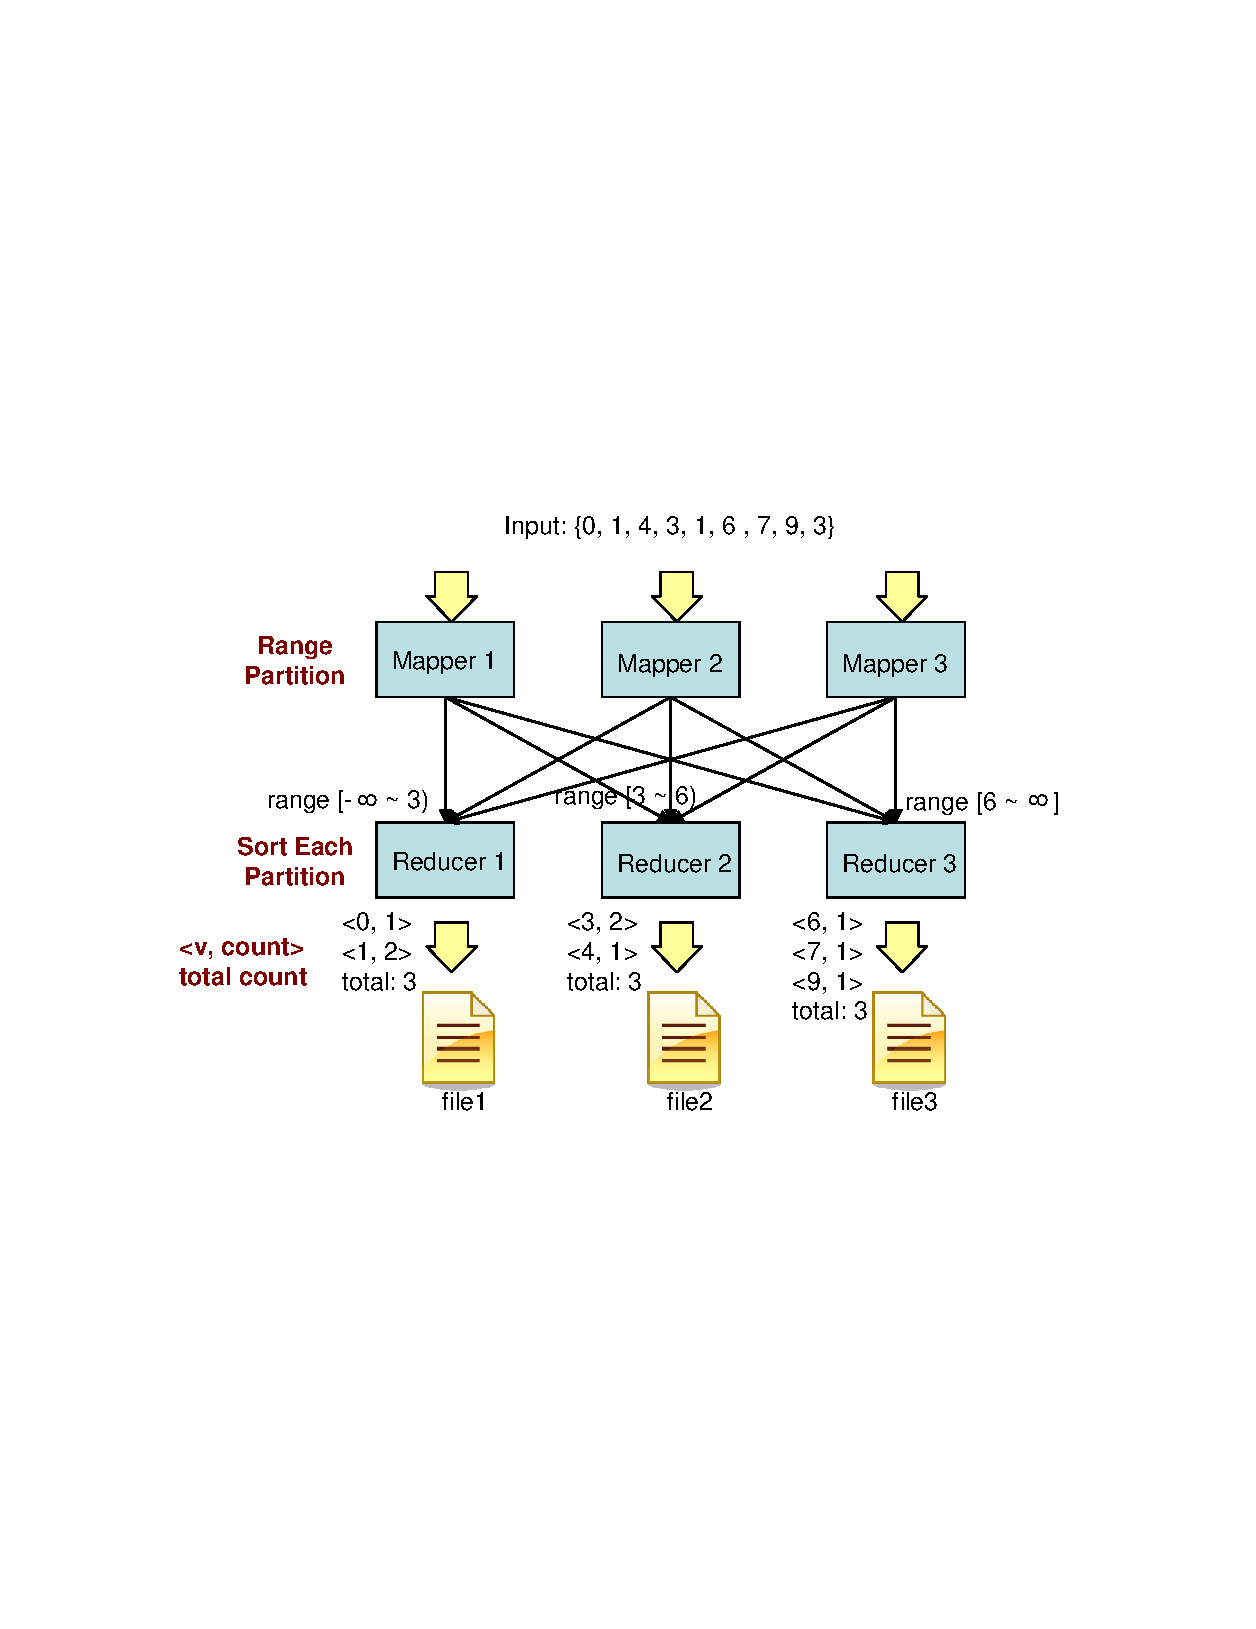
\includegraphics{figs/orderStats.eps}
%\caption{Sort-Based Order Statistics Algorithm}
%\label{fig:orderStats}
%\end{figure}

\textbf{Sort-Based Order Statistics Algorithm:} This algorithm consists of three phases. The first two phases are inspired by Yahoo's TeraSort algorithm~\cite{terasort}.

%This algorithm has the following three phases: (1) the sample phase to decide on the boundaries for range partitioning the data, (2) the sort phase to sort each range partition, and (3) the selection phase to select the order statistics. The first two phases are very similar to Yahoo's TeraSort algorithm~\cite{terasort}.

%\textit{Sample Phase}: This phase samples $N_s$ data items from the input data in a serial program. The $N_s$ samples are then sorted and divided evenly into $r$ partitions, where $r$ is the number of reducers allocated. The pivots of the sample partitions are used as the boundaries for range partitions in the next phase.

% more detailed description of the sampling phase.
%Given a specified number of samples $N_s$ and the proportion of the HDFS blocks to be touched for the sample $p$, this program randomly selects $p*B$ ($B$ is the number of HDFS blocks for the input data) blocks, and samples $N_s/(p*B)$ data items from each block. Then, the sample is sorted and divided evenly into $r$ partitions, where $r$ is the number of reducers allocated for the \textit{quantile} algorithm. The pivots of the sample partitions are used as the boundary for range partitioning the whole input for the next phase.


%\textit{Sort Phase}: This phase is implemented as a MapReduce job. The job reads the input data, and uses the results from the sample phase to range partition the input data, each reducer corresponding to one range. Each reducer sorts the unique values in their ranges and also keep a count for each unique value (a similar combiner is used to reduce the data shuffled to the reducers). In addition, each reducer computes the sum of all the counts (i.e. the number of data items) in its range.

%\textit{Selection Phase}: The sort phase produces $r$ sorted HDFS files, as well as the number of data items in each file. It is straightforward to derive which file contains a given order statistic. Locating the order statistic requires only scanning this file until the data item is found (early termination is possible). When multiple required order statistics reside in a single file, the scan cost can be shared. In addition, different files are scanned concurrently to improve further efficiency.

%Then, the algorithm scans the file until it finds the required data item(s). If multiple quantiles reside in the same HDFS file, the scan cost can be shared. When the input quantile vector $P$ is very large and the algorithm has to touch multiple HDFS files to compute all quantiles in $P$, we implement a special Hadoop InputFormat class to perform the selection phase, with each input split scans one file until all required data items are reached and feeds the quantiles directly to whatever jobs that use this input format. 

%\reminder{how about describing the way to do all columns at once? Not sure, because, right now the quantile is only defined on a vector}


\textit{Sample Phase}: This phase samples $N_s$ items from the input data, which are then sorted and divided evenly into $r$ partitions, where $r$ is the number of reducers. The boundary points are used for range partitioning in the next phase.

\textit{Sort Phase}: As shown in Figure~\ref{fig:orderStats}, this phase is a MapReduce job that reads the input data, and uses the results from the previous phase to range partition the data. Each range is assigned to a different reducer, which sorts the unique values and keeps the number of occurrences for each unique value. Each reducer also computes the total number of data items in its range.

%\textit{Selection Phase}: The output of sort phase ($r$ sorted HDFS files and their sizes) is be used to identify the appropriate file(s) for the required order statistic(s). If multiple statistics reside in a single file, the scan cost can be shared. Furthermore, different files are scanned concurrently for improved efficiency.

\textit{Selection Phase}: For a given set of required order statistics, the output of sort phase ($r$ sorted HDFS files and number of items in each file) is used to identify the appropriate file(s) that need to be scanned. If multiple order statistics reside in a single file, the scan cost can be shared. Furthermore, different files are scanned concurrently for improved efficiency.


%The sort phase produces $r$ sorted HDFS files, as well as the number of items in each file. It is straightforward to derive which file contains a given order statistic. Locating the order statistic requires only scanning this file until the data item is found (early termination is possible). When multiple required order statistics reside in a single file, the scan cost can be shared. In addition, different files are scanned concurrently to improve further efficiency.


\section{Experiments}
\label{sec:exp}
\subsection{Experimental Setup}\label{sec:exp-setup}

\textbf{Experiment Cluster}: The experiments were conducted with Hadoop 0.20~\cite{hadoop} on a cluster with 5 machines as worker nodes. Each machine has 8 cores with hyperthreading enabled, 32 GB RAM and 2 TB storage. We set each machine to run 15 concurrent mappers and 10 concurrent reducers.

\textbf{Experiment Data Sets}: There exist several benchmark data sets to assess the accuracy of numerical algorithms and software, such as NIST StRD~\cite{nist}. However, these benchmarks mostly provide very small date sets. For example, the largest data set in NIST StRD contains only 5000 data points. To test the numerical stability of distributed algorithms, we generated large synthetic data sets similar to those in NIST StRD. Our data generator takes the data size and the value range as inputs, and generates values from uniform distribution. For our experiments, we created data sets with different sizes (10million to 1billion) whose values are in the following 3 ranges, R1:[1.0 -- 1.5), R2:[1000.0 -- 1000.5) and R3:[1000000.0 -- 1000000.5).

\textbf{Accuracy Measurement}: In order to assess the numerical accuracy of the results produced by any algorithm, we need the true values of statistics. For this purpose, we rely on Java $BigDecimal$ that can represent arbitrary-precision signed decimal numbers. We implemented the naive algorithms for all statistics using Java $BigDecimal$ with precision $1000$. With such a high precision, results of all mathematically equivalent algorithms should approach closely to the true value. We implemented naive recursive summation for sum, sum divided by count for mean, one-pass algorithms for higher-order statistics as shown in Table~\ref{tab:1-pass}, and textbook one-pass algorithm for covariance. We consider obtained results as the ``true values" of these statistics.

We measure the accuracy achieved by different algorithms using the Log Relative Error (LRE) metric described in~\cite{LRE}. If $q$ is the computed value from an algorithm and $t$ is the true value, then LRE is defined as $$LRE=-\log_{10}|\frac{q-t}{t}|$$
LRE measures the number of significant digits that match between the computed value from the algorithm $q$ and the true value $t$. Therefore, a higher value of LRE indicates that the algorithm is numerically more stable.

%The higher a LRE value is, the better the algorithm. 
%is, the more desirable the estimated value is. As mentioned above, $t$ in our context refers to the values obtained using $BigDecimal$.

\begin{table}[tbh]
\caption{Textbook One-Pass Algorithms for Higher-Order Statistics}
\label{tab:1-pass}
\centering
\begin{tabular}{|c|c|}
\hline
& Equations for 1-Pass Algorithm \\
\hline
variance & $\frac{1}{n-1}S_2-\frac{1}{n(n-1)}S_1^2$ \\
\hline
std & $(variance)^{\frac{1}{2}}$ \\
\hline
skewness & $\frac{S_3 - \frac{3}{n}S_1S_2 + \frac{2}{n^2}S_1^3}{n\times std\times variance}$\\
\hline
kurtosis & $\frac{S_4 - \frac{4}{n}S_3S_1 + \frac{6}{n^2}S_2S_1^2 - \frac{3}{n^3}S_1^4}{n\times (variance)^2} - 3$ \\
\hline
%\multicolumn{2}{l}{}\\
\multicolumn{2}{c}{$S_p=\sum\limits_{i=1}^{n}x_i^p$, which can be easily computed in one pass.}
\end{tabular}
\end{table}

\subsection{Numerical Stability of Univariate Statistics}\label{sec:univariate_exp}

In this section, we demonstrate the numeric stability of SystemML in computing a subset of univariate statistics. 

\begin{table*}[thb]
\caption{Numerical Accuracy of Sum and Mean (LRE values)}
\label{tab:sum}
\centering
\begin{tabular}{|c|c|r|r|r|r|r|}
\hline
 & \textbf{Size} & \multicolumn{3}{|c|}{\textbf{Sum}} &  \multicolumn{2}{|c|}{\textbf{Mean}}\\
 & (million) & \multicolumn{3}{|c|}{} &  \multicolumn{2}{|c|}{}\\
\hline
\textbf{Range} & & SystemML & Naive & Sorted & SystemML & Naive\\ 
\hline
             & 10   & 16.1 & 13.5 & 16.1 & 16.7 & 13.5 \\
\textbf{R1}  & 100  & 16.3 & 13.8 & 13.6 & 16.2 & 13.8 \\
             & 1000 & 16.8 & 13.6 & 13.5 & 16.5 & 13.6 \\
\hline
\hline
             & 10   & 16.8 & 14.4 & 13.9 & 16.5 & 14.4 \\
\textbf{R2}  & 100  & 16.1 & 13.4 & 13.4 & 16.9 & 13.4 \\
             & 1000 & 16.6 & 13.1 & 13.9 & 16.4 & 13.1 \\
\hline
\hline
             & 10   & 15.9 & 14.0 & 13.9 & 16.3 & 14.0 \\
\textbf{R3}  & 100  & 16.0 & 13.1 & 13.4 & 16.9 & 13.1 \\
             & 1000 & 16.3 & 12.9 & 12.2 & 16.5 & 12.9 \\
\hline
\end{tabular}
\end{table*}

Table~\ref{tab:sum} lists the accuracy (LRE values) of results produced by different algorithms for sum and $mean$. For summation, we compare the MapReduce Kahan summation used in SystemML against the naive recursive summation and the sorted summation. The latter two algorithms are adapted to the MapReduce environment. In case of naive recursive summation, mappers compute the partial sums using recursive summation, which are then aggregated in the reducer. 
%This adapted naive recursive summation is used in both PIG and HIVE. 
In case of sorted summation, we first sort the entire data on MapReduce using the algorithm described in Section~\ref{sec:sort-order-stats}, and then apply the adapted naive recursive summation on the sorted data. As shown in Table~\ref{tab:sum}, SystemML consistently produces more accurate results than the other two methods. The accuracies from naive recursive summation and the sorted summation are comparable. In terms of runtime performance, our MapReduce Kahan summation and the naive recursive summation are similar, but the sorted summation is up to $5$ times slower as it performs an explicit sort on the entire data. Similarly, the accuracies obtained by SystemML for mean are consistently better than naive ``sum divided by count" method.

%We also compare the accuracy of mean algorithms in Table~\ref{tab:sum}. Again, the mean algorithm in SystemML consistently produces more accurate results than the naive approach (naive recursive sum divided by count).

\begin{table*}[thb]
\caption{Numerical Accuracy of Higher-Order Statistics (LRE values)}
\label{tab:univariate}
\centering
\begin{tabular}{|c|c|r|r|r|r|r|r|r|r|}
\hline
 & \textbf{Size} & \multicolumn{2}{|c|}{\textbf{Variance}} & \multicolumn{2}{|c|}{\textbf{Std}} & \multicolumn{2}{|c|}{\textbf{Skewness}} & \multicolumn{2}{|c|}{\textbf{Kurtosis}}\\
 & (million) & \multicolumn{2}{|c|}{} & \multicolumn{2}{|c|}{} & \multicolumn{2}{|c|}{} & \multicolumn{2}{|c|}{}\\
\hline
\textbf{Range} & & SystemML & Naive & SystemML & Naive & SystemML & Naive & SystemML & Naive\\ 
\hline
             & 10   & 16.0 & 11.3 & 15.9 & 11.6 & 16.4 & 7.5 & 15.3 & 9.8 \\
\textbf{R1}  & 100  & 16.2 & 11.5 & 16.8 & 11.8 & 14.9 & 7.1 & 15.6 & 9.3 \\
             & 1000 & 16.0 & 11.3 & 16.4 & 11.6 & 14.5 & 6.5 & 15.6 & 8.9 \\
\hline
\hline
             & 10   & 15.4 & 5.9  & 15.9 & 6.2  & 12.5 & 0   & 14.9 & 0 \\
\textbf{R2}  & 100  & 15.6 & 5.3  & 15.8 & 5.6  & 12.0 & 0   & 14.9 & 0 \\
             & 1000 & 16.2 & 4.9  & 16.4 & 5.2  & 12.1 & 0   & 15.2 & 0 \\
\hline
\hline
             & 10   & 14.4 & 0    & 14.7 & 0    & 9.1  & 0   & 12.6  & 0 \\
\textbf{R3}  & 100  & 12.9 & 0    & 13.2 & NA   & 9.0  & NA  & 13.2  & NA \\
             & 1000 & 13.2 & 0    & 13.5 & NA   & 9.4  & NA  & 12.9 & NA \\
\hline
%\multicolumn{10}{l}{}\\
\multicolumn{10}{c}{NA represents undefined standard deviation, skewness or kurtosis due to a negative value for variance.}
\end{tabular}
\end{table*}

The accuracy comparison for higher-order statistics is shown in Table~\ref{tab:univariate}. In SystemML, we employ the algorithms presented in Section~\ref{sec:highorder} to compute required central moments, which are then used to compute higher-order statistics. We compare SystemML against the naive textbook one-pass methods (see Table~\ref{tab:1-pass}). As shown in Table~\ref{tab:univariate}, SystemML attains more accurate results for all statistics. The difference between the two methods in case of higher-order statistics is much more pronounced than that observed for sum and mean from Table~\ref{tab:sum}. This is because the round-off and truncation errors get magnified as the order increases. It is important to note that for some data sets in ranges R2 and R3, the higher-order statistics computed by the naive method are grossly erroneous ($0$ digits matched). More importantly, in some cases, the naive method produced negative values for variance, which led to undefined values for standard deviation, skewness and kurtosis (shown as NA in Table~\ref{tab:univariate}). 

%It is clearly shown in Table~\ref{tab:univariate} that SystemML algorithms are significantly more stable than the textbook one-pass algorithms. The advantage of SystemML is much higher in the higher-order statistics than sum and mean, because errors get more amplified as the order increases. For some datasets in ranges R2 and R3, the higher order statistics are completely wrong (0 digits matched). In particular, the R3 100 million data set and R3 1 billion data set produce negative variance, which leads to undefined standard deviation, skewness and kurtosis (shown as NA in Table~\ref{tab:univariate}).

The value range has a considerable impact on the accuracy of univariate statistics. Even though R1, R2, and R3 have the same delta (i.e., the difference between minimum and maximum value), the accuracies obtained by all the algorithms drop as the magnitude of values increases. A popular technique to address this problem is to shift all the values by a constant, compute the statistics, and add the shifting effect back to the result. The chosen constant is typically the minimum value or the mean (computed or approximate). Chan {\em et al.} showed that such a technique helps in computing statistics with higher accuracy~\cite{variance}. 

%Although the delta (difference between min and max values) of each range is the same (0.5), all algorithms including stable ones present decreasing accuracy from R1, R2 to R3. This is because the 3 ranges have increasing means. If we know ahead of time some basic characteristics of a dataset, we can simply shift the data before computing the statistics, then add the shifting effect back to the results. For example, it has been shown in~\cite{variance} that to compute variance for a dataset with a large mean, substantial gains in accuracy can be achieved by shifting all the data by some approximation of the mean. Similarly, shifting can be applied to the other univariate statistics for increased accuracy.

%\begin{table*}[t]
%\caption{Numerical Accuracy of Univariate Statistics (LRE values)}
%\label{tab:univariate}
%\centering
%\begin{tabular}{|c|c|r|r|r|r|r|r|r|r|r|r|r|r|r|}
%\hline
% & \textbf{size} & \multicolumn{3}{|c|}{\textbf{sum}} &  \multicolumn{2}{|c|}{\textbf{mean}}& \multicolumn{2}{|c|}{\textbf{variance}} & \multicolumn{2}{|c|}{\textbf{std}} & \multicolumn{2}{|c|}{\textbf{skewness}} & \multicolumn{2}{|c|}{\textbf{kurtosis}}\\
% & (million) & \multicolumn{3}{|c|}{} &  \multicolumn{2}{|c|}{}& \multicolumn{2}{|c|}{} & \multicolumn{2}{|c|}{} & \multicolumn{2}{|c|}{} & \multicolumn{2}{|c|}{}\\
%\hline
%\textbf{Range} & & SystemML & naive & sorted & SystemML & naive & SystemML & 1-pass & SystemML & 1-pass & SystemML & 1-pass & SystemML & 1-pass\\ 
%\hline
%    & 10   & 16.1 & 13.5 & 16.1 & 16.7 & 13.5 & 13.5 & 11.3 & 13.8 & 11.6 & 13.0 & 7.5 & 13.7 & 9.8 \\
%\textbf{R1}  & 100  & 16.3 & 13.8 & 13.6 & 15.9 & 13.8 & 13.7 & 11.5 & 14.0 & 11.8 & 12.5 & 7.1 &  12.8 & 9.3 \\
%    & 1000 & 16.8 & 13.6 & 13.5 & 16.5 & 13.6 & 14.1 & 11.3 & 14.4 & 11.6 & 12.1 & 6.5 & 11.8 & 8.9 \\
%\hline
%\hline
%    & 10   & 16.8 & 14.4 & 13.9 & 16.5 & 14.4 & 12.8 & 5.9  & 13.1 & 6.2  & 11.8 & 0   & 13.4 & 0 \\
%\textbf{R2}  & 100  & 16.1 & 13.4 & 13.4 & 15.9 & 13.4 & 12.5 & 5.3  & 12.8 & 5.6  & 9.7  & 0   & 14.3 & 0 \\
%    & 1000 & 16.6 & 13.1 & 13.9 & 16.4 & 13.1 & 13.8 & 4.9  & 14.1 & 5.2  & 9.3  & 0   & 11.8 & 0 \\
%\hline
%\hline
%    & 10   & 15.9 & 14.0 & 13.9 & 15.7 & 14.0 & 9.3  & 0    & 9.6  & 0    & 7.1  & 0   & 9.5  & 0 \\
%\textbf{R3}  & 100  & 16.0 & 13.1 & 13.4 & 16.0 & 13.1 & 9.5  & 0    & 9.8  & NA   & 6.8  & NA  & 9.7  & 0 \\
%    & 1000 & 16.3 & 12.9 & 12.2 & 16.1 & 12.9 & 10.3 & 0    & 10.5 & NA   & 6.3  & NA  & 10.0 & 0 \\
%\hline
%\end{tabular}
%\end{table*}



\subsection{Numerical Stability of Bivariate Statistics}\label{sec:bivariate_exp}

We now discuss the numerical accuracy achieved by SystemML for bivariate statistics. We consider two types of statistics: {\em scale-categorical} and {\em scale-scale}. In the former type, we compute {\em Eta}\footnote{Eta is defined as $(1-\frac{\sum\limits_{r=1}^{R}(n_r-1)\sigma_r^2}{(n-1)\sigma^2})^{\frac{1}{2}}$, where $R$ is the number of categories, $n_r$ is the number of data entries per category, $\sigma_r^2$ is the variance per category, $n$ is the total number of data entries, and $\sigma^2$ is the total variance.} and {\em ANOVA-F}\footnote{ANOVA-F is defined as $\frac{\sum\limits_{r=1}^{R}n_r(\mu_r-\mu)^2}{\sum\limits_{r=1}^{R}(n_r-1)\sigma_r^2}.\frac{n-R}{R-1}$, where $R$ is the number of categories, $n_r$ is the number of data entries per category, $\mu_r$ is the mean per category, $\sigma_r^2$ is the variance per category, $n$ is the total number of data entries, and $\mu$ is the total mean.} measures, whereas in the latter case, we compute {\em covariance} and {\em Pearson correlation (R)}\footnote{Pearson-R is defined as $\frac{\sigma_{xy}}{\sigma_x\sigma_y}$, where $\sigma_{xy}$ is the covariance, $\sigma_x$ and $\sigma_y$ are standard deviations.}. For scale variables, we use data sets in value ranges R1, R2 and R3 that were described in Section~\ref{sec:exp-setup}. For categorical variables, we generated data in which $50$ different categories are uniformly distributed.

For computing these statistics, SystemML relies on numerically stable methods for {\em sum}, {\em mean}, {\em variance} and {\em covariance} from Section~\ref{sec:stability}, whereas the naive method in comparison uses the naive recursive summation for sum, sum divided by count for mean, and textbook one-pass algorithms for variance and covariance. 

The LRE values obtained for scale-categorical statistics are shown in Table~\ref{tab:bivar_sc}. From the table, it is evident that the statistics computed in SystemML have higher accuracy than the ones from the naive method. It can also be observed that the accuracy achieved by both methods reduces as the magnitude of input values increases -- e.g., LRE numbers for R3 are smaller than those of R1. As we move from R1 to R3, the accuracy of the naive method drops more steeply compared to SystemML. This is because the inaccuracies of total and per-category $mean$ and $variance$ quickly propagate and magnify the errors in Eta and ANOVA-F. 
%This emphasizes the fact that the use of inaccurate values in computations can lead to grossly erroneous results. 
Similar trends can be observed in case of covariance and Pearson correlation, as shown in Table~\ref{tab:bivar_ss}. For the cases of R2 vs. R3 with $100$ million and $1$ billion data sets, the naive algorithm produces negative values for variance (see Table~\ref{tab:univariate}), which resulted in undefined values for Pearson-R (shown as NA in Table~\ref{tab:bivar_ss}).

\begin{table}[t]
\centering
\caption{Numerical Accuracy of Bivariate Scale-Categorical Statistics: Eta and ANOVA-F (LRE values)}
\label{tab:bivar_sc}
\begin{tabular}{|c|c|r|r|r|r|}
\hline
 & \textbf{Size} & \multicolumn{2}{|c|}{\textbf{Eta}} &  \multicolumn{2}{|c|}{\textbf{ANOVA-F}} \\
 & (million) & \multicolumn{2}{|c|}{} &  \multicolumn{2}{|c|}{} \\
\hline
\textbf{Range} & & SystemML & Naive & SystemML & Naive \\ 
\hline
             & 10   & 16.2 & 13.7 & 16.2 & 10.0 \\
\textbf{R1}  & 100  & 16.6 & 13.7 & 15.6 & 10.0 \\
             & 1000 & 16.5 & 13.6 & 15.8 & 9.9  \\
\hline
\hline
             & 10   & 16.2 & 7.2 & 13.3 & 3.5 \\
\textbf{R2}  & 100  & 16.6 & 7.4 & 13.4 & 3.7 \\
             & 1000 & 16.5 & 7.9 & 13.4 & 4.3 \\
\hline
\hline
             & 10   & 16.2 & 0   & 10.2 & 0 \\
\textbf{R3}  & 100  & 15.9 & 1.9 & 10.0 & 0 \\
             & 1000 & 16.5 & 1.2 & 10.0 & 0 \\
\hline
\end{tabular}
\end{table}


\begin{table}[t]
\centering
\caption{Numerical Accuracy of Bivariate Scale-Scale Statistics: Covariance and Pearson-R (LRE values)}
\label{tab:bivar_ss}
\begin{tabular}{|c|c|r|r|r|r|}
\hline
 & \textbf{Size} & \multicolumn{2}{|c|}{\textbf{Covariance}} &  \multicolumn{2}{|c|}{\textbf{Pearson-R}} \\
 & (million) & \multicolumn{2}{|c|}{} &  \multicolumn{2}{|c|}{} \\
\hline
\textbf{Range} & & SystemML & Naive & SystemML & Naive \\ 
\hline
                     & 10   & 15.0 &  8.4 & 15.1 &  6.2 \\
\textbf{R1 vs. R2}   & 100  & 15.6 &  8.5 & 15.4 &  6.4 \\
                     & 1000 & 16.0 &  8.7 & 15.7 &  6.2 \\
\hline
\hline
                     & 10   & 13.5 &  3.0 & 13.5  & 3.0  \\
\textbf{R2 vs. R3}   & 100  & 12.8 &  2.8 & 12.7 & NA \\
                     & 1000 & 13.6 &  3.9 & 13.8 & NA \\
\hline
%\multicolumn{6}{l}{}\\
\multicolumn{6}{c}{NA represents undefined Pearson-R due to a negative value for variance.}
\end{tabular}
\end{table}






\subsection{The Impact of \textsc{KahanIncrement}}
\label{sec:comparison_exp}
In this section, we evaluate the effect of using \textsc{KahanIncrement} in the update rules of central moments (Equation~\ref{eq:cmeq}) and covariance (Equation~\ref{eq:coveq}) on the accuracy of the results.

Table~\ref{tab:univariate-vs-hive} and Table~\ref{tab:bivar_vs_hive} show the numerical accuracy achieved by the update rules using \textsc{KahanIncrement} and basic addition for higher-order statistics and scale-scale bivariate statistics. Evidently, update rules using \textsc{KahanIncrement} are able to produce more accurate results for all statistics across the board. In SystemML, the correction terms maintained in Kahan technique helps in reducing the effect of truncation errors. 

%The latest version of HIVE (0.7.1) provides a number descriptive statistics including \textit{sum}, \textit{mean}, \textit{variance}, \textit{standard deviation}, \textit{covariance}, and \textit{pearson correlation}. We now compare the accuracies achieved by SystemML against those of HIVE, for several statistics. Since HIVE (as well as PIG) computes \textit{sum} and \textit{mean} using the naive recursive summation algorithm, the comparison between SystemML and HIVE on these two statistics will be same as the results presented in Table~\ref{tab:sum}. 
%
%For higher order statistics, covariance, and Pearson correlation, both SystemML and HIVE employ the same incremental update rules, as shown in Sections~\ref{sec:highorder}~\&~\ref{sec:covariance}. The primary difference is that SystemML makes use of \textsc{KahanIncrement} to perform aggregations, whereas HIVE relies on the basic addition. The differences in accuracy achieved by SystemML and HIVE are shown in Table~\ref{tab:univariate-vs-hive} and Table~\ref{tab:bivar_vs_hive}. Evidently, SystemML is able to produce more accurate results than HIVE for all statistics across the board. In SystemML, the correction terms maintained in Kahan technique helps in reducing the effect of truncation errors.

%As discussed in Section~\ref{sec:highorder} and Section~\ref{sec:covariance}, HIVE employs similar update rule as in SystemML to compute variance, standard deviation, covariance and pearson correlation. However, SystemML uses \textsc{KahanIncrement} in the update rule, whereas HIVE just employs the basic addition. In Table~\ref{tab:univariate-vs-hive} and Table~\ref{tab:bivar_vs_hive}, we compare the accuracy of results produced by the algorithms used in SystemML and HIVE. For both univariate and bivariate statistics, it is evident that SystemML presents significant advantage over HIVE.

%\begin{table}[thb]
%\caption{Accuracy Comparision between SystemML and HIVE for Variance and Standard Deviation (LRE values)}
%\label{tab:univariate-vs-hive}
%\centering
%\begin{tabular}{|c|c|r|r|r|r|}
%\hline
% & \textbf{Size} & \multicolumn{2}{|c|}{\textbf{Variance}} & \multicolumn{2}{|c|}{\textbf{Std}} \\
% & (million) & \multicolumn{2}{|c|}{} & \multicolumn{2}{|c|}{}\\
%\hline
%\textbf{Range} & & SystemML & HIVE & SystemML & HIVE \\ 
%\hline
%             & 10   & 16.0 & 13.5 & 15.9 & 13.8  \\
%\textbf{R1}  & 100  & 16.2 & 13.7 & 16.8 & 14.0  \\
%             & 1000 & 16.0 & 14.1 & 16.4 & 14.4  \\
%\hline
%\hline
%             & 10   & 15.4 & 12.8  & 15.9 & 13.1   \\
%\textbf{R2}  & 100  & 15.6 & 12.5  & 15.8 & 12.8   \\
%             & 1000 & 16.2 & 13.8  & 16.4 & 14.1   \\
%\hline
%\hline
%             & 10   & 14.4 & 9.3    & 14.7 & 9.6     \\
%\textbf{R3}  & 100  & 12.9 & 9.5    & 13.2 & 9.8    \\
%             & 1000 & 13.2 & 10.3   & 13.5 & 10.6    \\
%\hline
%\end{tabular}
%\end{table}

\begin{table*}[thb]
\caption{The Effect of \textsc{KahanIncrement} on the Accuracy of Higher-Order Statistics (LRE values)}
\label{tab:univariate-vs-hive}
\centering
\begin{tabular}{|c|c|r|r|r|r|r|r|r|r|}
\hline
 & \textbf{Size} & \multicolumn{2}{|c|}{\textbf{Variance}} & \multicolumn{2}{|c|}{\textbf{Std}} & \multicolumn{2}{|c|}{\textbf{Skewness}} & \multicolumn{2}{|c|}{\textbf{Kurtosis}}\\
 & (million) & \multicolumn{2}{|c|}{} & \multicolumn{2}{|c|}{} & \multicolumn{2}{|c|}{} & \multicolumn{2}{|c|}{}\\
\hline
\textbf{Range} & & Kahan & Basic & Kahan & Basic & Kahan & Basic & Kahan & Basic\\ 
\hline
             & 10   & 16.0 & 13.5 & 15.9 & 13.8 & 16.4 & 13.0 & 15.3 & 13.7 \\
\textbf{R1}  & 100  & 16.2 & 13.7 & 16.8 & 14.0 & 14.9 & 12.5 & 15.6 & 12.8 \\
             & 1000 & 16.0 & 14.1 & 16.4 & 14.4 & 14.5 & 12.1 & 15.6 & 11.8\\
\hline
\hline
             & 10   & 15.4 & 12.8  & 15.9 & 13.1  & 12.5 & 11.8  & 14.9 & 13.4 \\
\textbf{R2}  & 100  & 15.6 & 12.5  & 15.8 & 12.8  & 12.0 & 9.7   & 14.9 & 14.3 \\
             & 1000 & 16.2 & 13.8  & 16.4 & 14.1  & 12.1 & 9.3   & 15.2 & 11.8 \\
\hline
\hline
             & 10   & 14.4 & 9.3    & 14.7 & 9.6  & 9.1  & 7.1   & 12.6  & 9.5 \\
\textbf{R3}  & 100  & 12.9 & 9.5    & 13.2 & 9.8  & 9.0  & 6.8  & 13.2  & 9.7 \\
             & 1000 & 13.2 & 10.3   & 13.5 & 10.6 & 9.4  & 6.3  & 12.9 & 10.0 \\
\hline
\end{tabular}
\end{table*}



\begin{table}[t]
\centering
\caption{The Effect of \textsc{KahanIncrement} on the Accuracy of Covariance and Pearson-R (LRE values)}
\label{tab:bivar_vs_hive}
\begin{tabular}{|c|c|r|r|r|r|}
\hline
 & \textbf{Size} & \multicolumn{2}{|c|}{\textbf{Covariance}} &  \multicolumn{2}{|c|}{\textbf{Pearson-R}} \\
 & (million) & \multicolumn{2}{|c|}{} &  \multicolumn{2}{|c|}{} \\
\hline
\textbf{Range} & & Kahan & Basic & Kahan & Basic \\ 
\hline
                     & 10   & 15.0 &  14.2 & 15.1 &  13.0 \\
\textbf{R1 vs. R2}   & 100  & 15.6 &  13.3 & 15.4 &  13.0 \\
                     & 1000 & 16.0 &  14.6 & 15.7 &  14.2 \\
\hline
\hline
                     & 10   & 13.5 &  10.0 & 13.5  & 9.8  \\
\textbf{R2 vs. R3}   & 100  & 12.8 &  10.0 & 12.7 & 10.5 \\
                     & 1000 & 13.6 &  11.4 & 13.8 & 10.5 \\
\hline
\end{tabular}
\end{table}


\subsection{Performance of Order Statistics}

In this section, we evaluate the scalability of the sort-based order statistics algorithm presented in Section~\ref{sec:sort-order-stats}. Script~\ref{scpt:linearrg} shows how order statistics are expressed in DML language -- more details on the DML syntax can be found in~\cite{systemml}. The script computes the median as well as other quantiles as specified by the vector $P$, from the input data $V$. In this experiment, we fix $P=\{0.1, 0.2, 0.3, 0.4, 0.5, 0.6, 0.7, 0.8, 0.9\}$, and vary the size of $V$ (the value range of data in $V$ is R1). Figure~\ref{fig:orderStatsScale} shows the execution time of this script as the input data size increases. For the given DML script, SystemML is able to identify that multiple different order statistics are computed on the same data set, and it accordingly performs a single sort and then computes the required order statistics. Furthermore, all the specified order statistics are selected simultaneously, in parallel.

\
\begin{script}\label{scpt:linearrg}
A Simple Script of Order Statistics\\
\footnotesize
\texttt{
1:\ \ \# input vector (column matrix)\\
2:\ \ V = read("in/V");\\
3:\ \ \# a vector specifying the desired quantiles \\
4:\ \ P = read("in/P");\\
5:\ \ \# compute median\\
6:\ \ median = quantile(V, 0.5);\\
7:\ \ print("median: ", median);\\
8:\ \ \# compute quantiles\\
9:\ \ Q = quantile(V, P);\\
10:\ write(Q, "out/Q");\\}
\end{script}

\onefigure
{figs/order_stats_scale.eps}
{Execution Time for Script 1}
{fig:orderStatsScale}






\section{Discussion}
We now summarize the lessons learned while implementing scalable and numerically stable descriptive statistics in SystemML.
\\

\noindent $\bullet$ \textbf{Many existing sequential techniques for numerical stability can be adapted to the distributed environment.} 

We successfully adapted the existing sequential stable algorithms for summation, mean, central moments and covariance to the MapReduce environment. Such adaptations are empirically shown to exhibit better numeric stability when compared to commonly used naive algorithms.
\\

\noindent $\bullet$ \textbf{Performance need not be sacrificed for accuracy.} 

While software packages like $BigDecimal$ can be used to improve the numerical accuracy of computations, they incur significant performance overhead -- we observed up to 5 orders of magnitude slowdown depending on the exact operation and precision used. Similarly, the {\em sorted sum} technique that is widely used in sequential environments is not able to achieve similar accuracy when adapted to a distributed environment. Furthermore, its performance is hindered by the fact that the entire data has be sorted up front. In contrast, our stable algorithms for summation, mean, covariance, and higher order statistics achieve good accuracy without sacrificing the runtime performance -- they make a single scan over the input data, and achieve comparable runtime performance with the unstable one-pass algorithms.
\\

%Although BigDecimal provides the flexibility to use any algorithms for accurate results, it incurs substantial performance overhead (up to 5 orders of magnitude slowdown depending on the precision observed in our study). Our stable summation, central moments and covariance algorithms only perform one pass over data, and achieve comparable performance to the corresponding unstable one-pass algorithms. The sorted summation algorithm, although a common practice in the sequential environment, is inferior to our stable summation method in terms of both performance and accuracy.

\noindent $\bullet$ \textbf{Shifting can be used for improved accuracy.} 

When all the values in the input data set are of large magnitude, it is useful to shift the elements by a constant (minimum value or approximate mean) prior to computing any statistics. This preprocessing technique helps in reducing the truncation errors, and often achieves better numerical accuracy. In the absence of such preprocessing, as shown in Sections~\ref{sec:univariate_exp}~\&~\ref{sec:bivariate_exp}, the accuracy of statistics degrades as the magnitude of input values increases (e.g., as the value range changes from R1 to R3).
\\

%Through the experiments in Section~\ref{sec:univariate_exp} and Section~\ref{sec:univariate_exp}, we observed that for a same delta, ranges with higher means suffer from degraded accuracies. However, by shifting all the data by an approximation of mean before attempting to compute descriptive statistics, significant gains of accuracy can be achieved.

%\noindent $\bullet$ \textbf{Divide-and-conquer improves the boundary of numerical stability for large data.} 
\noindent $\bullet$ \textbf{Divide-and-conquer design helps in scaling to larger data sets while achieving good numerical accuracy.} 

All the stable algorithms discussed in this paper operate in a divide-and-conquer paradigm, in which the partial results are computed in the mappers and combined later in the reducer. These algorithms partitions the work into smaller pieces, and hence they can scale to larger data sets while keeping the relative error bound independent of the input data size. For example, the sequential version of Kahan summation algorithm guarantees that the relative error bound is independent of the input data size as long as the {\em total number} of elements is in the order of $10^{16}$. In contrast, the MapReduce version of Kahan summation algorithm can provide similar guarantees as long as the data size processed by {\em each} mapper is in the order of $10^{16}$. In the words, the parallel version of the algorithm can scale to larger data sets without having a significant impact on the error bound. Here, we assume that the number of mappers is bounded by a constant which is significantly smaller than the input data size. While there is no formal proof of such a result for covariance and other higher-order statistics, we expect the distributed algorithms for these statistics to scale better than their sequential counterparts.
\\

%For the MapReduce Kahan summation algorithm, we have derived an error bound with higher boundary of numerical stability in Section~\ref{sec:sum}. More specifically, for sequential Kahan summation, the upper bound of data size that can be processed stably is in the order $10^{16}$. By applying the divide-and-conquer strategy, the MapReduce Kahan summation, has a much higher bound: as long as each mapper process less than the order of $10^{16}$ data entries. Although we don't have formal proof for the MapReduce central moments and covariance algorithms, we expect them to present similar trend.

\noindent $\bullet$ \textbf{Kahan technique is useful beyond a simple summation.} 

The strategy of keeping the correction term, as in Kahan summation algorithm, helps in alleviating the effect of truncation errors. Beyond the simple summation, we found this technique to be useful in computing stable values for other univariate and bivariate statistics, including mean, variance, covariance, Eta, ANOVA-F etc.



\section*{Acknowledgment}
We would like to thank Peter Haas for his valuable suggestions and consultation on this work. We would also like to thank the other members of the SystemML team: Douglas R. Burdick, Amol Ghoting, Rajasekar Krishnamurthy, Edwin Pednault, Vikas Sindhwani, and Shivakumar Vaithyanathan.

\bibliographystyle{abbrv}
\bibliography{ref}

\newpage

%\appendix
\begin{appendices}
\section{Proof of Error Bound for MapReduce Kahan Summation Algorithm}
The relative error bound for the MapReduce Kahan summation algorithm is $\frac{|E_n|}{|S_n|}\leq [4u+4u^2+O(mu^2)+O(\frac{n}{m}u^2)+O(mu^3)+O(\frac{n}{m}u^3)+O(nu^4)]\condnumber $.

\begin{proof}
As each of the $m$ mappers uses Kahan algorithm, the $k$-th mapper has the error bound $E_{n_k}=|\hat{S}_{n_k}-S_{n_k}|\leq (2u+O(n_ku^2))\sum\limits_{i=1}^{n_k}|x_{k,i}|$, where $n_k$ is the number of data items process by this mapper. As $n_k$ is in $O(\frac{n}{m})$, we can simply derive $E_{n_k}\leq(2u+O(\frac{n}{m}u^2))\sum\limits_{i=1}^{n_k}|x_{k,i}|$.

Each mapper generates $\hat{S}_{n_k}$ with its correction term. In the single reducer, we again run the Kahan sum algorithm on these $m$ data items, therefore, we get derive the error incurred in the reducer as follows:
{
\footnotesize
\begin{align}
&|\hat S_n-\sum\limits_{i=1}^{m}\hat{S}_{n_k}| \nonumber\\
 \leq & (2u+O(mu^2))\sum\limits_{k=1}^{m}|\hat{S}_{n_k}| \nonumber\\
 \leq & (2u+O(mu^2))\sum\limits_{k=1}^{m}(|S_{n_k}|+ E_{n_k})\nonumber\\
 \leq & (2u+O(mu^2))\sum\limits_{k=1}^{m}(\sum\limits_{i=1}^{n_k}|x_{k,i}|+ (2u+O(\frac{n}{m}u^2))\sum\limits_{i=1}^{n_k}|x_{k,i}|) \nonumber \\
\leq & (2u+O(mu^2))(1+2u+O(\frac{n}{m}u^2))\sum\limits_{i=1}^n|x_i| \nonumber \\
\leq & (2u+4u^2+O(mu^2)+O(mu^3)+O(\frac{n}{m}u^3)+O(nu^4))\sum\limits_{i=1}^n|x_i| \nonumber
\end{align}
}

We can now derive the upper bound on the relative error for MapReduce Kahan summation as follows:
{
\footnotesize
\begin{align}
\small 
&|\hat S_n-S_n| = |\hat S_n-\sum\limits_{i=1}^{m}S_{n_k}|\nonumber\\
= &|\hat S_n-\sum\limits_{i=1}^{m}\hat{S}_{n_k}+\sum\limits_{i=1}^{m}\hat{S}_{n_k}-\sum\limits_{i=1}^{m}S_{n_k}|\nonumber\\
\leq & |\hat S_n-\sum\limits_{i=1}^{m}\hat{S}_{n_k}|+|\sum\limits_{i=1}^{m}\hat{S}_{n_k}-\sum\limits_{i=1}^{m}S_{n_k}|\nonumber\\
\leq & |\hat S_n-\sum\limits_{i=1}^{m}\hat{S}_{n_k}|+\sum\limits_{i=1}^{m}|\hat{S}_{n_k}-S_{n_k}|\nonumber\\
\leq & |\hat S_n-\sum\limits_{i=1}^{m}\hat{S}_{n_k}| + \sum\limits_{i=1}^{m}((2u+O(\frac{n}{m}u^2))\sum\limits_{i=1}^{n_k}|x_{k,i}|)\nonumber\\
\leq & (2u+4u^2+O(mu^2)+O(mu^3)+O(\frac{n}{m}u^3)+O(nu^4))\sum\limits_{i=1}^n|x_i| \nonumber\\
& + (2u+O(\frac{n}{m}u^2))\sum\limits_{i=1}^n|x_i| \nonumber \\
\leq & (4u+4u^2+O(mu^2)+O(\frac{n}{m}u^2)+O(mu^3)+O(\frac{n}{m}u^3)+O(nu^4))\sum\limits_{i=1}^n|x_i|\nonumber
\end{align}
}

As a result, the relative error bound for MapReduce Kahan summation is $\frac{|E_n|}{|S_n|}\leq [4u+4u^2+O(mu^2)+O(\frac{n}{m}u^2)+O(mu^3)+O(\frac{n}{m}u^3)+O(nu^4)]\condnumber $. 
\end{proof}

\end{appendices}

\end{document}
